\documentclass{article}
\usepackage[utf8]{inputenc}

\title{Online voting: measure of privacy and verifiability}
\author{boire.sebastien }
\date{November 2020}

\usepackage{natbib}
\usepackage{graphicx}
\usepackage{amsmath}
\usepackage{amssymb}


\newcommand{\Prob}{\mathbb{P}}

\begin{document}

\maketitle


\section{Definitions of privacy and verifiability}

\subsection{Quantifying information on a vote}

If we have access to some partial information on a vote, we want to measure the mount of information we can get from it. From a message mes, we define a function quantifying the information on the message as:

$Info(mes)=\dfrac{\text{number of possible votes coherent with mes}}{\text{total number of possible votes}}$

This definition can be applied to the vote of one user, with a receipt providing partial information on the vote, but also on an entire election, with mes being all the public information we have access to.


\subsection{Privacy}

Privacy is the amount of money required to buy one vote, taking into account the probability that the vote was correctly bought. For instance, if 10€ are given to any person who has a proof such that "I voted for candidate A or candidate B", with candidate A being the one that we want to buy, then privacy amounts to 20€. (This holds true if the voter cannot choose A and B appearing in his proof, but only chooses who he votes for).


$privacy=\dfrac{\text{cost to change one vote}}{\text{probability that the vote was performed according to the attacker's will}}$


\subsection{Verifiability}

The election can be verified using all the public information on the votes. We define verifiability as:

$Verifiability=Info(\text{all public receipts})*\text{level of verification}$

The level of verification is the probability with which the verification confirms the result of the election.


\section{First scheme: public storage of a subset of possible vote values}

\subsection{Description}

We consider an election with candidates $C_1, ..., C_K$. Voter V votes for $C_i$, and the value of the vote is stored encrypted so that it can be counted, verified by V, and secret. In addition, (k-1) other candidates are chosen at random, and a public ticket is produced: "Voter V voted for $C_{i_1}$ or $C_{i_2}$ or ... or $C_{i_k}$.", with one of the $C_{i_j}$ being $C_i$, the correct value.

\subsection{Evaluation of verifiability}

We note $X^i_j$ the binary variable corresponding to "Does voter j voted for candidate i?". Then:

$Y_\alpha^i=X^i_1+...+X^i_\alpha$ is a binomial variable following $\mathcal{B}(\alpha, p_i)$, with $p_i$ probability of vote for candidate i.

In a similar way, we note $\tilde{X}^i_j$ the binary variable corresponding to "Does the public vote of voter j contains candidate i as a possible vote?".

$\tilde{Y}_\alpha^i=\tilde{X}^i_1+...+\tilde{X}^i_\alpha$ is a binomial variable following $\mathcal{B}(\alpha, \tilde{p}_i)$, with $\tilde{p}_i$ probability that candidate i is in a public vote.

We have:

$\tilde{p}_i=p_i+(1-p_i)*\frac{k-1}{K-1}$


We use Bienayme-Tchebychev inequality on $\tilde{Y}_\alpha^i$:

$ \mathbb{P}(|\dfrac{\tilde{Y}^i_\alpha-\alpha*\tilde{p}_i}{\alpha}| > x )  \leqslant \dfrac{\tilde{p}_i(1-\tilde{p}_i)}{\alpha x^2}$


Using the public votes of $\alpha$ voters, we can compare the scores we obtain for each candidate to the global results of the election, and measure whether the difference is likely or not. This provides a measure of verifiability (we just need to choose a level of verification with the term $\dfrac{\tilde{p}_i(1-\tilde{p}_i)}{\alpha x^2}$).


\subsection{Evaluation of privacy}

Privacy can be defined in multiple ways. Here, we will measure the entropy on one vote, as the amount of unknown information to an attacker to know one vote.

$Privacy=H(vote)=-\sum\limits_{c \in candidates} p(c)log_2(p(c))=log_2(k)$

In this, we do not take into account that each candidate has a probability $p_i$ of being the real value of the vote (to simplify calculations). This corresponds to the situation where each candidate obtains as much vote as any other.


\section{Second scheme: public storage of the votes under probabilistic value}


\subsection{Description}

The election is in the same configuration as in the previous section. However, before the the voter chooses who he votes for, he sees a set of random variables appearing on the screen: $R_1, ..., R_K$. They all follow a Gaussian law, with $R_1$ following a $\mathcal{N}(\mu, \sigma^2)$, and all the other $R_i$ following a $\mathcal{N}(\frac{1-\mu}{K}, \sigma^2)$. Then, the voter chooses who he votes for, and the variables $R_i$ are rotated so that $R_1$ is associated to the candidate chosen by the voter. The values of the $R_i$ are then made public. 

$\mu$ is chosen such that $\mu > \frac{1-\mu}{K}$, so that on average we can distinguish the correct candidate. The bigger the difference, the easier it is to identify the real value of the vote. In addition, $\sigma$ quantifies the randomness of the values of $R_i$, and also takes part in how easy it is to identify the real value of a vote.

\bigbreak

This structure allows the voter to be sure that he is not duped on the value of his public vote, since the random variables $R_i$ are evaluated before the voter enters his vote.

\bigbreak

For simplicity, $R_1$ is chosen to be $1-(R_2+\cdots+R_K)$ such that the sum results in 1.


\subsection{Privacy evaluation}

An attacker who wants to buy votes will rely on the public receipt of the vote, which only contains partial information. Therefore, the attacker will pay an amount proportional to $R_j$.

We suppose that the voter wants to vote for $C_1$, and the attacker wants the voter to vote for $C_j$, $j\neq 1$. The attacker will consider that the user voted for the candidate associated to the highest of the $R_i$s. We need to measure the frequency that the highest of the $R_i$s is associated to $C_1$, revealing the correct vote. The parameters that can be modified are:
\begin{itemize}
    \item $\epsilon$: this defines the mean for the distribution of $R_1$, as $\mu + \epsilon$. $\epsilon$ determines how confident the verification can be.
    \item $\sigma$: the highest the sigma, the more dense the distributions. $\sigma$ determines how many votes are necessary for the result of the verification to be trustworthy.
\end{itemize}

We generate random sets of $R_1, \cdots, R_K$, and measure the probability that each one is associated to both distribution. We note $D_1$ the distribution of $R_1$ (correct value of the vote), and $D_2$ the distribution of the incorrect values of the vote (for $R_2, \cdots, R_K$).

We have:

$\mathbb{P}(R_i\text{ follows }D_1 | \text{1 of the Rs follows }D_1)=\dfrac{\mathbb{P}(R_i\sim D_1)\mathbb{P}(R_1 \sim D_2)\cdots \mathbb{P}(R_K \sim D_2)}{\sum\limits_{j=1}^{K}\mathbb{P}(R_j\sim D_1)\mathbb{P}(R_1 \sim D_2)\cdots \mathbb{P}(R_K \sim D_2)}$

We count the number of times that $\mathbb{P}(R_i\text{ follows }D_1 | \text{1 of the Rs follows }D_1)$ is maximum for i=1 as the number of times the correct vote of the user is revealed to the attacker. Ideally, it should happen 1/K times.

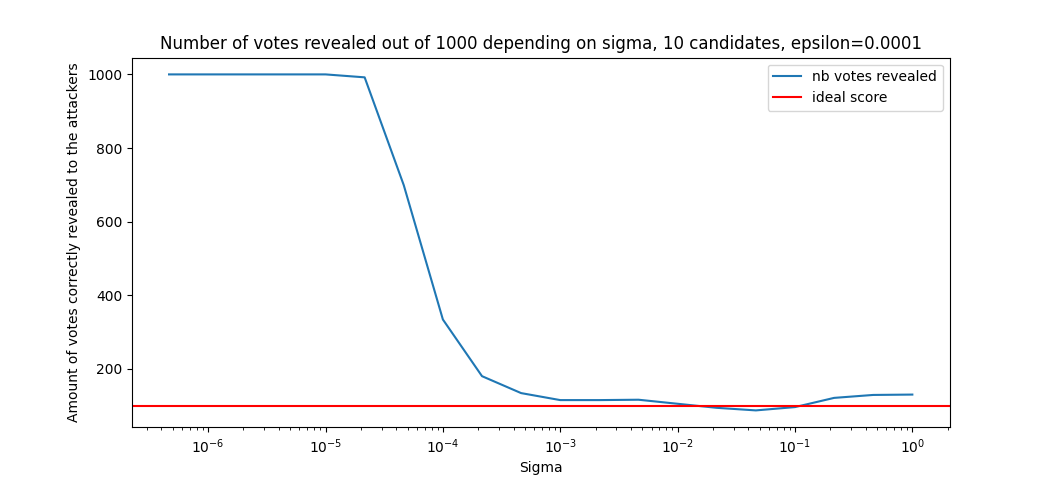
\includegraphics[scale=0.5]{distribution_proba/influence_sigma.png}
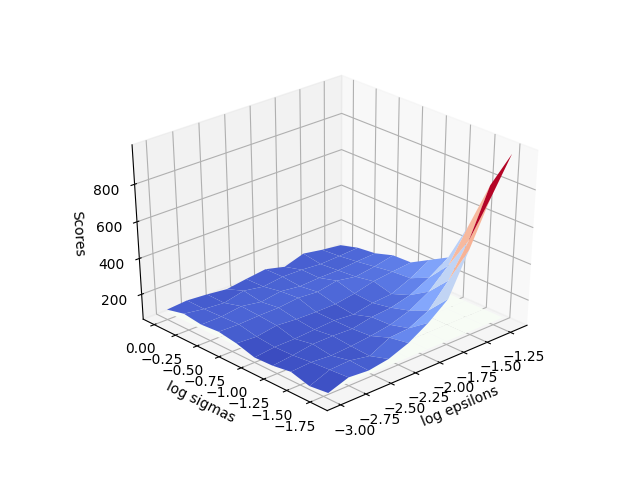
\includegraphics[scale=0.8]{distribution_proba/influence_sigma_epsilon.png}


From the graph, we see that complete privacy is reachable for some correct choices of $(\sigma, \epsilon)$: $\sigma$ must be big enough, $\epsilon$ must be small enough.

\subsection{Verifiability evaluation}


We are going to measure the verifiability by playing on $\sigma, \epsilon$ again. However, this time we measure something else: the resulting distribution probability of the election result. The election result is the percentage of votes for $C_1$ that we estimate (in reality, it is 100\%).However, a key parameter is the number of votes: the bigger the number of voters, the better the verification is.

\bigbreak

Let's suppose that the public ticket of voter $V_i$ is $(R_1(V_i), \cdots, R_K(V_i))$ with a real vote for $C_1$ for all users. We consider that $R_2, \cdots, R_K$ follow the probability distribution $\mathcal{N}(\mu ,\sigma)$, and $R_1$ follows the probability distribution $\mathcal{N}(\mu+\epsilon ,\sigma)$. We suppose that the sum is normalized such that for each user: $R_1 + \cdots + R_K=1$.

Knowing only the public tickets, the probability that the voter voted for each candidates are:

$\Prob(V_i: C_k)=\dfrac{R_k(V_i) - \mu}{\epsilon}$

Hence $Prob(V_i: C_k)$ follows the probability distribution $\mathcal{N}(0, \dfrac{\sigma}{\epsilon})$ for $k>1$, and $Prob(V_i: C_1)$ follows the probability distribution $\mathcal{N}(1, \dfrac{\sigma}{\epsilon})$.

From this, we note $Res(C_k)$ the predicted result of candidate $C_k$ from the public tickets:

$Res(C_k)=\sum\limits_{V_i}\dfrac{p_k(V_i)-\mu}{\sigma}$

Hence:

$Res(C_1) \sim \mathcal{N}(N, \dfrac{\sigma \sqrt{N}}{\epsilon})$

$Res(C_k) \sim \mathcal{N}(0, \dfrac{\sigma \sqrt{N}}{\epsilon})$

Hence the precision of the verifiability is proportionate to $\dfrac{\sigma \sqrt{N}}{\epsilon}$. From the initial definitions:

$Info(\text{1 ticket})=\epsilon$

$Info(\text{all tickets})=N \epsilon$

$Verif=N \epsilon * \dfrac{\sigma \sqrt{N}}{\epsilon} = N\sqrt{N} \sigma$.

Beware: this measure of verification is limited, since it does not result in $\epsilon$ in its measure. Maybe $\dfrac{\sigma \sqrt{N}}{\epsilon}$ is better?

\underline{Interpretation: } If we consider a population of 1 million voters, and (according to the privacy section) $\dfrac{\sigma}{\epsilon}=10^{1.25}$, we have a result of election confirmed with a precision of less than 1700 votes in 66\% of cases, and 3400 votes in 98\% of cases. This is a precision of 1.7\% (respectively 3.4\%): it is good, but can in some conditions not be enough.

\section{Protection against corruption within the administrators}

\subsection{Description}

The administrators (state, government, authorities, ...) have access to all the results of the votes: they are able to tamper with it at will in a way that is coherent with the public receipts. Therefore, some protection is necessary. It takes several steps:
\begin{itemize}
    \item after the election is over: the administrators publish a list containing all the votes (code(voter), vote). The code(voter) is the result of hash(pk(voter), confidential\_code(voter)), where confidential\_code(voter) is a random number generated by the admins after the elections, kept secret even from the voter himself. This list will be called S1.
    \item during the election: when a voter votes, the administrators store the vote in their private database. At the same time, the voter is presented with an assertion of type "I voted for candidates $C_{i_1}$ or $C_{i_2}$ or $C_{i_3}$ or $C_{i_4}$", generated automatically by a program, that is coherent with the vote of the user. The administrator encrypts it with his public key, the voter then encrypts the result with his public key, and the result is stored on a public registry that cannot be tampered, even by the administrators (blockchain-like). This registry will be called S2.
    
    This way, this secret assertion can only be verified with the participation of both the voter and the administrator. In addition, the administrator does not know the content of this assertion. 
    
    \item after the election: a small proportion of the population are chosen at random (randomness can be ensured in a trusted way). Only those voters can perform the following operation.
    
    If willing, they can go to a specific place, and request the verification of their vote: the administrator gives them confidential\_code(voter), so that the voter can look at the value of his vote in the public list of votes. At this point, he knows what his vote was, but it may have been tampered by the administrator. Then, with the participation of the administrator, he decrypts his assertion from S2, and checks whether it is compatible with the value from S1. If incompatible, then he has proof of corruption. 
\end{itemize}

In order for this to work, we need to be sure that hash(pk(voter), confidential\_code(voter)) has enough randomness, but also enough restrictions so that the administrator cannot create a convenient confidential\_code(voter) on request to fit the hash with any vote in S1. Therefore, we need the length of hash(pk(voter), confidential\_code(voter)) to be much longer than the length of confidential\_code(voter). In addition, we also need enough complexity so that there cannot be brute-force attack from the voter to verify his vote without the participation of the administrator: the lenght of confidential\_code(voter) has to be big enough.


\bigbreak

This technique is sufficient to prevent corruption of the vote, but there may be some difficulties in the population to accept it as enough verifiability: indeed, the proportion of individuals that can perform this verification is small, in order to prevent an outsider from paying the voters and then requesting them to provide proof. Therefore, the population relies on a small proportion of the voters to state that the election was honest. 


\section{Third scheme: Privacy of the votes depending on subgroups of the voting population}

\end{document}
 
